\sloppy

\documentclass[12pt,a4paper]{report}

\usepackage[utf8]{inputenc}
\usepackage[T1]{fontenc}
\usepackage[french]{babel}
\usepackage{graphicx}
\usepackage{geometry}
\geometry{margin=2.5cm}
\usepackage[backend=biber,style=numeric]{biblatex}
\usepackage{csquotes}
\addbibresource{references.bib}
\usepackage{float}
\usepackage{algorithm}
\usepackage{algorithmic}
\usepackage{amsmath}
\graphicspath{{images/}}

\begin{document}
\begin{titlepage}
    \centering
    
    % Université
    \textsc{\LARGE Université Moulay Slimane}\\[0.5cm]
    \textsc{\Large FST}\\[0.5cm]
    \textsc{\large Département : Informatique}\\[2cm]
    
    % Logo (optionnel)
    % \includegraphics[width=0.3\textwidth]{logo.png}\\[1cm]
    
    \textsc{\Large Rapport de PFE}\\[1.5cm]
    
    % Titre
    {\Huge \bfseries Optimisation du Computation Offloading dans les réseaux MEC à l’aide du MARL\\[0.5cm]}
    
    \vfill
    
    % Réalisé par
    \textbf{Réalisé par :}\\
    AIT AHMED OULHAJ SOULAIMANE \\[1cm]
    
    % Encadrants
    \textbf{Encadré par :}\\
    Pr. AIT OMAR DRISS\\[1cm]
    
    % Année
    \textbf{Année Universitaire :} 2024 -- 2025
    
\end{titlepage}

\tableofcontents
\newpage

\listoffigures
\newpage

\section*{Summary of Notation}

\begin{table}[H]
\centering
\renewcommand{\arraystretch}{1.3}
\begin{tabular}{|c|l|}
\hline
\textbf{Symbole} & \textbf{Description} \\
\hline
$\mathcal{N}$ & Ensemble des agents (devices IoT générateurs de tâches) \\
$\mathcal{M}$ & Ensemble des dispositifs (IoT, Edge, Cloud) \\
$\mathcal{L}_n$ & Ensemble des couches de la tâche $n$ \\
$L_n$ & Nombre total de couches de la tâche $n$ \\
$A_{n,l}^m$ & Variable de décision (1 si la couche $l$ est exécutée sur $m$) \\
$c_{n,l}$ & Coût de calcul de la couche $l$ \\
$m_{n,l}$ & Besoin mémoire de la couche $l$ \\
$D_{n,l}$ & Taille des données de sortie de la couche $l$ \\
$T_n$ & Latence totale de la tâche $n$ \\
$E_n$ & Énergie totale consommée pour la tâche $n$ \\
$T_{comp}(n,l,m)$ & Temps de calcul de la couche $l$ sur le dispositif $m$ \\
$T_{comm}(n,l,m',m)$ & Temps de communication entre deux dispositifs \\
$E_{comp}(n,l,m)$ & Énergie de calcul \\
$E_{comm}(n,l,m',m)$ & Énergie de communication \\
$F_m$ & Fréquence CPU du dispositif $m$ \\
$BW_m$ & Bande passante du dispositif $m$ \\
$C^{mem}_m$ & Capacité mémoire du dispositif $m$ \\
$B_m$ & Budget énergétique du dispositif $m$ \\
$TR_m$ & Score de confiance du dispositif $m$ \\
$\sigma_{n,l}$ & Niveau de confidentialité de la couche $l$ \\
$\alpha, \beta$ & Coefficients de pondération (latence / énergie) \\
$f_{eff}$ & Fréquence effective (DVFS) \\
$\rho$ & Ratio de fréquence (DVFS) \\
$\kappa$ & Constante matérielle (modèle CMOS) \\
$P_{comp}$ & Puissance de calcul \\
$P_{comm}$ & Puissance de communication \\
$W_{comp}$ & Délai d’attente (CPU) \\
$W_{comm}$ & Délai d’attente (réseau) \\
\hline
\end{tabular}
\caption{Summary of notation used in this work}
\label{tab:notation}
\end{table}

\chapter*{Introduction Générale}

Au cours de la dernière décennie, l’Internet des Objets (IoT) s’est imposé comme l’un des piliers majeurs de la transformation numérique \cite{mecsurvey}. Des milliards de dispositifs connectés, tels que les capteurs intelligents, les objets portables (\textit{wearables}), les véhicules autonomes et les systèmes industriels, sont aujourd’hui déployés dans divers domaines, notamment la santé, les villes intelligentes, l’industrie 4.0 et les transports intelligents. Ces dispositifs génèrent en continu de grandes quantités de données hétérogènes, nécessitant un traitement rapide et efficace.

Parallèlement, les avancées en intelligence artificielle, en particulier dans le domaine du \textit{Deep Learning}, ont permis de concevoir des modèles capables d’extraire des connaissances complexes à partir de grandes quantités de données \cite{rlpdnn2021}. Ces modèles sont utilisés dans des applications critiques telles que la reconnaissance d’images, la détection d’objets, la surveillance intelligente et la prise de décision autonome. Toutefois, ces modèles sont généralement gourmands en ressources de calcul et en mémoire, ce qui rend leur déploiement difficile sur des dispositifs IoT à capacités limitées.

Traditionnellement, le traitement des données est effectué dans des infrastructures distantes disposant de fortes capacités de calcul \cite{mecsurvey}. Bien que cette approche permette de bénéficier d’une puissance de traitement importante, elle introduit plusieurs contraintes, notamment des délais de transmission élevés, une consommation accrue de bande passante, ainsi qu’une dépendance à la connectivité réseau.

Afin de pallier ces limitations, le paradigme du \textit{Edge Computing} a émergé \cite{baccour2024}. Il consiste à rapprocher les ressources de calcul et de stockage des sources de données, en déployant des capacités de traitement au niveau du réseau périphérique ou directement sur des nœuds intermédiaires. Cette approche permet de réduire les délais de communication, d’améliorer la réactivité du système et de limiter la surcharge du réseau.

Cependant, malgré ces avantages, l’exécution des applications intelligentes dans des environnements distribués reste un défi complexe \cite{mi2024}. En effet, les dispositifs impliqués présentent des capacités hétérogènes en termes de calcul, d’énergie et de connectivité. De plus, les applications modernes, telles que la réalité augmentée, la conduite autonome et les systèmes critiques, nécessitent des décisions en temps réel, imposant des contraintes strictes en termes de latence.

Dans ce contexte, la gestion efficace de l’exécution des tâches devient un enjeu central. Il est nécessaire de déterminer dynamiquement où et comment exécuter les tâches (localement ou sur des nœuds proches), tout en optimisant l’utilisation des ressources disponibles et en respectant les contraintes de performance.

Ainsi, la problématique principale de ce travail s’inscrit dans le cadre de l’optimisation de l’allocation et de l’exécution des tâches dans des environnements distribués, en tenant compte des contraintes de latence, de ressources limitées et de dynamique du système. Cette problématique ouvre la voie à l’exploration de méthodes intelligentes, notamment basées sur l’apprentissage par renforcement, afin de prendre des décisions adaptatives dans des environnements complexes et incertains \cite{baccour2024}.

Dans ce travail, nous adoptons une approche basée sur l’apprentissage par renforcement multi-agent (MARL), où chaque dispositif IoT est modélisé comme un agent autonome capable d’interagir avec son environnement et de prendre des décisions concernant l’exécution locale ou le déchargement des tâches vers les nœuds Edge. Cette approche permet de développer des stratégies adaptatives prenant en compte la dynamique du système et les contraintes multiples telles que la latence, l’énergie et la disponibilité des ressources.

L’objectif principal de ce mémoire est de proposer une approche intelligente basée sur le MARL afin d’optimiser l’allocation et l’exécution des tâches dans les environnements Edge Computing. Plus précisément, il s’agit de minimiser la latence, de réduire la consommation énergétique, d’améliorer l’utilisation des ressources disponibles et de garantir la sécurité ainsi que la confidentialité des données.

\section*{Organisation du mémoire}

Ce mémoire est structuré comme suit :

\begin{itemize}
    \item \textbf{Chapitre 1 : Cadre Général du Projet} \\
    Ce chapitre présente le contexte général, la problématique, les motivations ainsi que les objectifs du projet.

    \item \textbf{Chapitre 2 : État de l’Art} \\
    Ce chapitre propose une analyse des travaux existants relatifs à l’Edge Computing, au task offloading, ainsi qu’aux approches basées sur le reinforcement learning et le MARL.

    \item \textbf{Chapitre 3 : Modélisation et Méthodologie} \\
    Ce chapitre décrit la modélisation du problème, la définition des agents, des états, des actions et de la fonction de récompense dans le cadre du MARL.

    \item \textbf{Chapitre 4 : Résultats et Discussion} \\
    Ce chapitre expose les résultats expérimentaux obtenus et leur analyse comparative avec les approches existantes.

    \item \textbf{Chapitre 5 : Conclusion et Perspectives} \\
    Ce chapitre conclut le travail et présente les perspectives futures de recherche.
\end{itemize}

\chapter{Cadre Général du Projet}

\section{Problématique}

Malgré les avancées apportées par les architectures distribuées et le traitement en périphérie, plusieurs défis majeurs persistent dans l’exécution des applications intelligentes dans les environnements IoT.

Premièrement, les dispositifs impliqués sont fortement contraints en termes de ressources, notamment en puissance de calcul, en capacité mémoire et en énergie. Ces limitations rendent difficile l’exécution locale de modèles d’intelligence artificielle complexes, en particulier ceux basés sur le \textit{Deep Learning}. De plus, la disponibilité des ressources peut varier dynamiquement en fonction des conditions du système, ce qui complique davantage la gestion de l’exécution des tâches \cite{liu2020marl}.

Deuxièmement, le transfert et le traitement des données dans des environnements distribués introduisent des contraintes importantes en termes de latence et de bande passante. Dans les applications critiques nécessitant des réponses en temps réel, tout retard dans la prise de décision peut entraîner une dégradation des performances ou des risques pour la sécurité \cite{kang2017neurosurgeon}.

Troisièmement, les aspects liés à la sécurité et à la confidentialité des données constituent un enjeu majeur. En effet, la distribution des tâches et des modèles d’apprentissage sur plusieurs nœuds peut exposer des informations sensibles, notamment en cas de présence de nœuds non fiables ou malveillants. Il devient alors nécessaire de limiter l’exposition des données et des modèles afin de prévenir toute tentative de reconstruction ou d’inférence non autorisée \cite{baccour2024,rlpdnn2021}.

Par ailleurs, la nature dynamique et hétérogène des environnements IoT rend les approches traditionnelles d’optimisation difficilement applicables. Les décisions concernant l’allocation des tâches doivent être prises de manière adaptative, en tenant compte de multiples contraintes simultanées telles que la latence, l’énergie, la disponibilité des ressources et les exigences de sécurité \cite{mi2024,liu2020marl}.

Ainsi, la problématique principale de ce travail consiste à concevoir une approche intelligente capable d’optimiser l’allocation et l’exécution des tâches dans un environnement distribué, tout en respectant des contraintes multiples, notamment la minimisation de la latence et de la consommation énergétique, ainsi que la garantie de la sécurité et de la confidentialité des données.

Dans ce contexte, l’apprentissage par renforcement multi-agent (MARL) apparaît comme une solution prometteuse, permettant de modéliser le problème comme un processus de décision séquentiel et de développer des stratégies adaptatives dans des environnements complexes et incertains \cite{mi2024,baccour2024}.

\section{Motivation}

La motivation principale de ce travail repose sur les limites des architectures traditionnelles basées sur le Cloud face aux exigences des applications IoT modernes. En effet, des applications telles que la réalité augmentée, les véhicules autonomes ou les systèmes de surveillance intelligente nécessitent des traitements en temps réel avec des contraintes strictes de latence.

Cependant, le modèle centralisé du Cloud introduit des délais de communication importants en raison de l’éloignement des centres de données, ce qui peut entraîner des performances insuffisantes dans les applications sensibles \cite{kang2017neurosurgeon}. Par ailleurs, les approches existantes présentent des limitations en termes de scalabilité, de coordination entre agents et de prise en compte simultanée de multiples contraintes.

Dans ce contexte, l’Edge Computing apparaît comme une solution pertinente en rapprochant les ressources de calcul des sources de données, permettant ainsi de réduire la latence, d’optimiser l’utilisation de la bande passante et d’améliorer la réactivité des systèmes \cite{mecsurvey}. De plus, le traitement local des données contribue à renforcer la confidentialité et la sécurité \cite{baccour2024}.

En outre, les environnements IoT sont dynamiques et hétérogènes, caractérisés par une variation continue des ressources disponibles. Cela rend les approches statiques inefficaces et nécessite des solutions adaptatives.

Dans ce cadre, l’apprentissage par renforcement multi-agent (MARL) constitue une approche prometteuse, permettant de modéliser les dispositifs IoT comme des agents autonomes capables d’apprendre des politiques optimales dans un environnement distribué. Cette approche est particulièrement adaptée aux problèmes d’allocation de ressources et de \textit{task offloading}, où plusieurs entités doivent prendre des décisions simultanées dans des conditions incertaines \cite{liu2020marl}.

Ainsi, la combinaison de l’Edge Computing et du MARL offre une solution efficace pour répondre aux contraintes de latence, d’énergie et de sécurité dans les systèmes IoT distribués.

\section{Contribution}

Dans ce contexte, ce travail vise à proposer une approche basée sur l’apprentissage par renforcement multi-agent (MARL) pour résoudre le problème d’allocation des tâches dans les environnements Edge-IoT. Contrairement aux approches classiques, notre solution repose sur une prise de décision distribuée, où chaque agent apprend de manière autonome tout en tenant compte de l’état global du système.

L’originalité de ce travail réside dans l’intégration simultanée des contraintes de latence, d’énergie et de sécurité dans un cadre MARL, permettant ainsi de développer une stratégie adaptative et efficace dans des environnements dynamiques et incertains.

\section{Objectif du Projet}

L’objectif principal de ce projet est de concevoir une approche intelligente basée sur l’apprentissage par renforcement multi-agent (MARL) afin d’optimiser l’allocation et l’exécution des tâches dans un environnement Edge Computing.

Plus précisément, ce travail vise à :

\begin{itemize}
    \item \textbf{Minimiser la latence} : réduire le temps de réponse des applications en rapprochant le traitement des données des dispositifs IoT.
    
    \item \textbf{Optimiser la consommation énergétique} : prolonger la durée de vie des dispositifs en réduisant les coûts énergétiques liés au calcul et à la communication.
    
    \item \textbf{Améliorer l’utilisation des ressources} : exploiter efficacement les capacités disponibles au niveau des nœuds Edge et des dispositifs.
    
    \item \textbf{Garantir la sécurité et la confidentialité} : limiter l’exposition des données sensibles et protéger les modèles d’apprentissage distribués.
    
    \item \textbf{Assurer l’adaptabilité du système} : développer une solution capable de s’ajuster dynamiquement aux changements de l’environnement (charge réseau, disponibilité des ressources, etc.).
\end{itemize}

Pour atteindre ces objectifs, le problème sera modélisé comme un processus de décision séquentiel, où chaque agent apprendre des politiques optimales concernant l’exécution locale ou le déchargement des tâches vers les nœuds Edge.


\section{Conclusion}

Dans ce chapitre, nous avons présenté le cadre général du projet en mettant en évidence les défis majeurs liés à l’exécution des applications intelligentes dans les environnements IoT distribués.

Nous avons montré que les approches traditionnelles basées sur le Cloud présentent des limitations importantes en termes de latence, de consommation de ressources et de sécurité. L’émergence de l’Edge Computing permet de répondre à ces défis en rapprochant le traitement des données des sources, améliorant ainsi la réactivité et l’efficacité des systèmes.

Cependant, la gestion optimale des ressources dans ces environnements reste un problème complexe en raison de leur nature dynamique et hétérogène. Dans ce contexte, l’apprentissage par renforcement multi-agent apparaît comme une solution pertinente pour concevoir des stratégies adaptatives et distribuées.

Ainsi, ce travail s’inscrit dans une démarche visant à exploiter les capacités du MARL pour optimiser l’allocation des tâches dans les systèmes Edge-IoT.

Le chapitre suivant sera consacré à l’état de l’art, où nous analyserons les différentes approches proposées dans la littérature pour le task offloading, l’allocation de ressources et l’utilisation du reinforcement learning dans les environnements Edge Computing.

\chapter{État de l’Art}

\section{Introduction}

Avec l’émergence des applications IoT nécessitant des traitements en temps réel, le paradigme du Edge Computing s’est imposé comme une solution prometteuse pour réduire la latence et améliorer les performances des systèmes distribués. Dans ce contexte, le problème du computation offloading a suscité un intérêt croissant, notamment avec l’intégration des techniques d’apprentissage automatique telles que le Reinforcement Learning (RL) et le Multi-Agent Reinforcement Learning (MARL). Ce chapitre présente une revue des travaux existants relatifs à ces domaines.


\section{Edge Computing}

\begin{figure}[H]
\centering
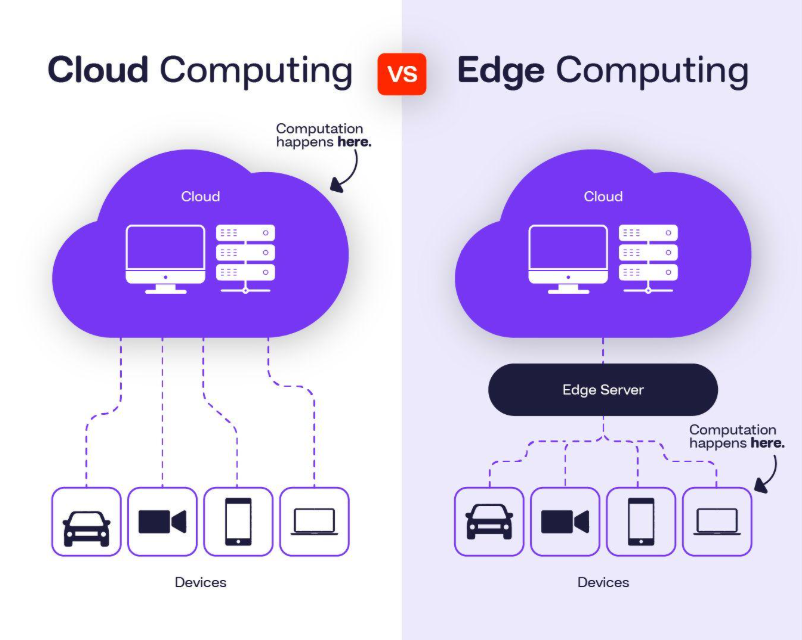
\includegraphics[width=0.8\textwidth]{edge_architecture.png}
\caption{Architecture de l’Edge Computing}
\end{figure}

La figure illustre la différence entre le Cloud Computing et l’Edge Computing. Dans le modèle Cloud, les données générées par les dispositifs IoT sont envoyées vers des centres de données distants pour être traitées, ce qui introduit une latence élevée.

L’Edge Computing est un paradigme distribué qui consiste à traiter les données au plus près de leur source, plutôt que de les envoyer vers des centres de données distants. Cette approche permet d’exécuter des opérations de calcul, de stockage et d’analyse directement au niveau des dispositifs périphériques ou des nœuds intermédiaires.

En rapprochant le traitement des données des dispositifs IoT, l’Edge Computing réduit considérablement le temps de transmission et améliore la réactivité des systèmes. Cette architecture est particulièrement adaptée aux applications nécessitant des décisions en temps réel, telles que les véhicules autonomes, la santé connectée ou les systèmes industriels intelligents.

\subsection{Avantages de l’Edge Computing}

\begin{figure}[H]
\centering
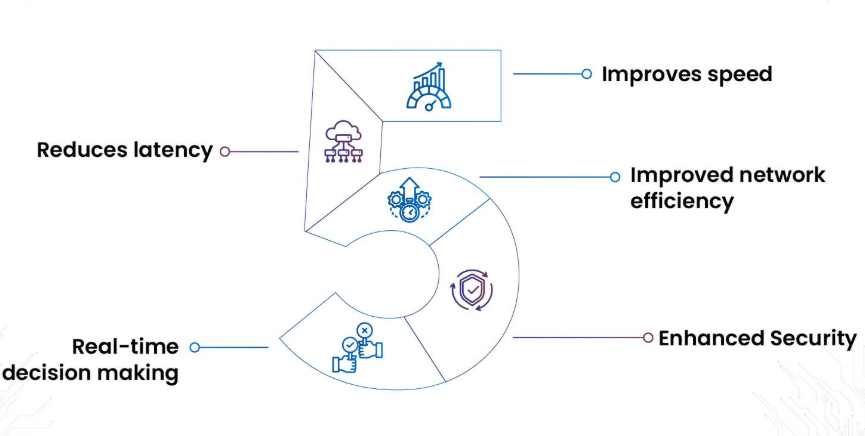
\includegraphics[width=0.7\textwidth]{edge_benefits.png}
\caption{Avantages de l’Edge Computing}
\end{figure}

L’Edge Computing offre plusieurs avantages majeurs dans les environnements IoT :

\begin{itemize}
    \item \textbf{Réduction de la latence :} Le traitement local des données permet de réduire le temps de réponse en évitant l’envoi vers des serveurs distants.
    
    \item \textbf{Amélioration des performances en temps réel :} Les décisions peuvent être prises rapidement, ce qui est essentiel pour les applications critiques.
    
    \item \textbf{Optimisation de la bande passante :} Seules les données pertinentes sont transmises vers le Cloud, réduisant ainsi le trafic réseau.
    
    \item \textbf{Sécurité et confidentialité :} Le traitement local limite l’exposition des données sensibles.
    
    \item \textbf{Fiabilité :} Le système peut continuer à fonctionner même en cas de perte de connexion avec le Cloud.
\end{itemize}

\subsection{Enjeux et défis}
Malgré ses nombreux avantages, l’Edge Computing présente plusieurs défis :

\begin{itemize}
    \item \textbf{Ressources limitées :} Les nœuds Edge disposent de capacités de calcul et de stockage limitées.
    
    \item \textbf{Sécurité :} La multiplication des dispositifs augmente les risques de cyberattaques.
    
    \item \textbf{Complexité de gestion :} La gestion d’un grand nombre de nœuds distribués est difficile.
    
    \item \textbf{Coût :} Le déploiement et la maintenance de l’infrastructure Edge peuvent être coûteux.
    
    \item \textbf{Scalabilité et coordination :} Assurer la coordination entre plusieurs nœuds reste un défi majeur, notamment dans les systèmes multi-agents.
\end{itemize}

\section{Computation Offloading}

Le computation offloading est un paradigme de calcul distribué qui consiste à transférer des tâches computationnelles intensives depuis des dispositifs à ressources limitées, tels que les objets IoT ou les smartphones, vers des infrastructures plus puissantes, notamment les serveurs Edge ou Cloud \cite{lin2020,offloading_general}. Cette approche permet de surmonter les contraintes liées à la capacité de calcul, au stockage et à l’énergie des dispositifs mobiles.

\subsection{Architecture du Computation Offloading}

\begin{figure}[H]
\centering
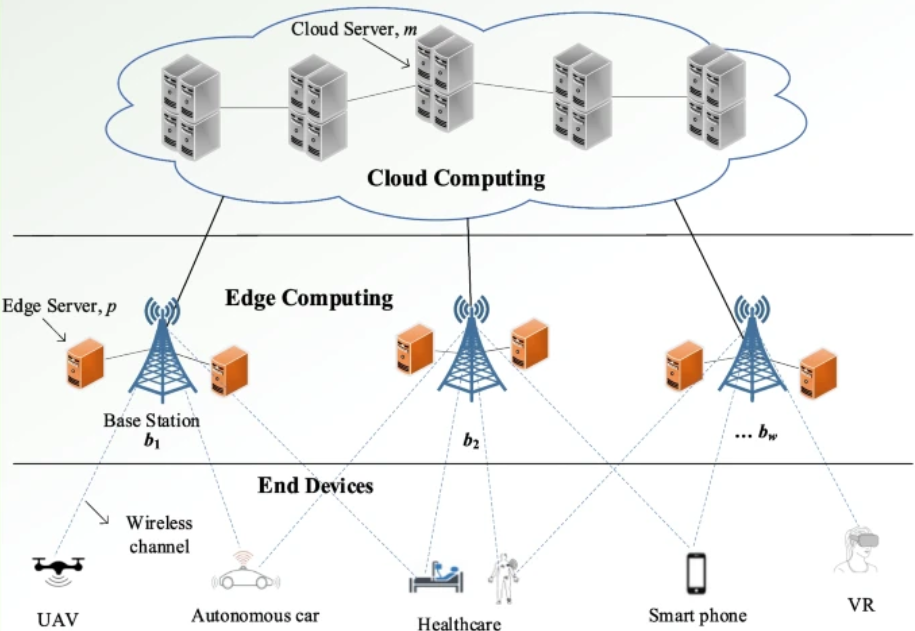
\includegraphics[width=0.85\textwidth]{offloading_architecture.png}
\caption{Architecture à trois niveaux du computation offloading (Edge Devices, Edge Nodes, Cloud)}
\end{figure}

Selon \cite{lin2020}, le computation offloading s’inscrit dans une architecture hiérarchique composée de trois couches principales :

\begin{itemize}
    \item \textbf{Edge Devices :} dispositifs IoT et terminaux mobiles générant les données.
    \item \textbf{Edge Nodes :} infrastructures intermédiaires (cloudlets, stations de base, micro data centers) offrant des capacités de calcul proches des utilisateurs.
    \item \textbf{Cloud :} centres de données distants fournissant une puissance de calcul élevée.
\end{itemize}

Cette architecture permet de distribuer dynamiquement les tâches entre les différents niveaux afin d’optimiser les performances et de réduire la latence.

\subsection{Processus du Computation Offloading}

Le processus de computation offloading comprend généralement trois étapes principales \cite{lin2020} :

\begin{enumerate}
    \item \textbf{Application Partitioning :} division de l’application en plusieurs composants exécutables localement ou à distance.
    \item \textbf{Offloading Decision :} détermination du lieu optimal d’exécution (local, Edge ou Cloud).
    \item \textbf{Execution Distribuée :} exécution des tâches sur les ressources sélectionnées.
\end{enumerate}

\subsection{Analyse du Computation Offloading}

Le computation offloading repose sur un compromis entre le gain de performance et le coût de communication. Il est bénéfique lorsque le temps d’exécution locale est supérieur au temps total de l’offloading, incluant la transmission et l’exécution distante \cite{lin2020}.

\begin{equation}
T_{local} > T_{offloading} = T_{communication} + T_{remote}
\end{equation}

De plus, l’énergie consommée pour la transmission doit être inférieure à celle de l’exécution locale, afin de garantir un gain énergétique.

\section{Reinforcement Learning}

Le Reinforcement Learning (RL) est une technique d’apprentissage automatique dans laquelle un agent apprend à prendre des décisions optimales en interagissant avec un environnement dynamique \cite{sutton2018}. Contrairement aux approches supervisées, le RL repose sur un mécanisme d’essai-erreur, où l’agent améliore progressivement sa politique à partir des récompenses reçues.

\subsection{Markov Decision Process (MDP)}

Le RL est généralement modélisé comme un processus de décision markovien (MDP), qui constitue un cadre mathématique pour la prise de décision séquentielle dans des environnements incertains \cite{sutton2018}.

\begin{figure}[H]
\centering
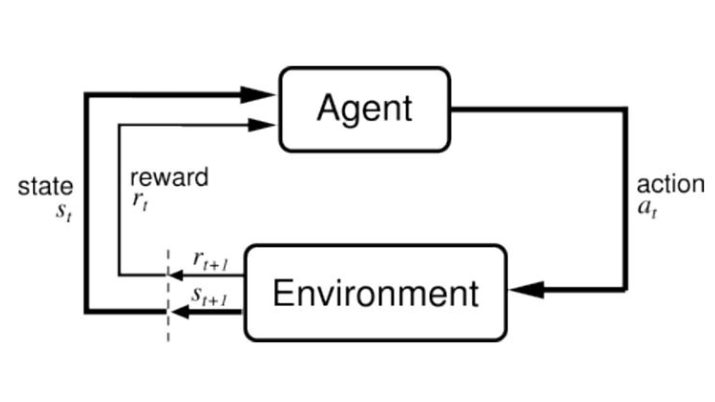
\includegraphics[width=0.7\textwidth]{MDP.png}
\caption{Interaction entre l'agent et son environnement}
\end{figure}

Un MDP est défini par le tuple $(S, A, P, R, \gamma)$.

\begin{itemize}
    \item $S$ : ensemble des états possibles,
    \item $A$ : ensemble des actions disponibles,
    \item $P(s'|s,a)$ : fonction de transition représentant la probabilité de passer à l’état $s'$,
    \item $R(s,a,s')$ : fonction de récompense,
    \item $\gamma$ : facteur de réduction des récompenses futures.
\end{itemize}

Le MDP repose sur la propriété de Markov, selon laquelle l’état futur dépend uniquement de l’état courant et de l’action choisie, et non de l’historique complet.

\subsection{Types de Reinforcement Learning}

Les méthodes de Reinforcement Learning peuvent être classées en deux grandes catégories : les approches basées sur la valeur et celles basées sur la politique.

\subsubsection{Value-Based Methods}

Les méthodes basées sur la valeur cherchent à estimer la fonction de valeur d’action $Q(s,a)$, qui représente la qualité d’une action donnée dans un état donné. L’agent choisit alors l’action qui maximise cette valeur :

\begin{equation}
a = \arg\max Q(s,a)
\end{equation}

Des algorithmes tels que le Q-learning et le Deep Q-Network (DQN) appartiennent à cette catégorie. Ces méthodes sont efficaces pour des espaces d’actions discrets, mais présentent des limitations dans des environnements complexes ou continus.

\subsubsection{Policy-Based Methods}

Les méthodes basées sur la politique apprennent directement une politique $\pi(a|s)$, qui définit la probabilité de choisir une action donnée dans un état donné :

\begin{equation}
\pi(a|s)
\end{equation}

Ces approches, telles que les méthodes de gradient de politique, sont particulièrement adaptées aux espaces d’actions continus et aux environnements complexes. Cependant, elles peuvent souffrir d’une variance élevée et nécessitent souvent un grand nombre d’échantillons pour converger.

\subsubsection{Approches hybrides (Actor-Critic)}

Les méthodes Actor-Critic combinent les avantages des approches précédentes en utilisant deux composants :
\begin{itemize}
    \item un \textbf{acteur} qui apprend la politique,
    \item un \textbf{critique} qui évalue les actions.
\end{itemize}

Ces méthodes permettent d’améliorer la stabilité et les performances de l’apprentissage, et sont largement utilisées dans les environnements complexes.

\subsection{Apprentissage par Q-learning}

Le Q-learning est une méthode populaire du RL qui met à jour les valeurs $Q(s,a)$ selon :

\begin{equation}
Q(s,a) \leftarrow Q(s,a) + \alpha \left[r + \gamma \max_{a'} Q(s',a') - Q(s,a)\right]
\end{equation}

où $\alpha$ est le taux d’apprentissage.

\subsection{Exploration vs Exploitation}

L’agent doit trouver un compromis entre :
\begin{itemize}
    \item l’exploration de nouvelles actions,
    \item l’exploitation des connaissances acquises.
\end{itemize}

Une stratégie courante est la méthode $\epsilon$-greedy.

\subsubsection{Pseudo-code du Q-learning}

\begin{algorithm}[H]
\caption{Q-learning}
\begin{algorithmic}[1]

\STATE Initialiser la Q-table $Q(s,a)$ arbitrairement
\STATE Définir le taux d’apprentissage $\alpha$ et le facteur de réduction $\gamma$

\FOR{chaque épisode}
    \STATE Initialiser l’état $s$
    
    \FOR{chaque étape}
    
        \STATE Choisir une action $a$ selon une politique $\epsilon$-greedy
        
        \STATE Exécuter l’action $a$
        
        \STATE Observer la récompense $r$ et le nouvel état $s'$
        
        \STATE Mettre à jour la valeur Q :
        \[
        Q(s,a) \leftarrow Q(s,a) + \alpha \left[r + \gamma \max_{a'} Q(s',a') - Q(s,a)\right]
        \]
        
        \STATE Mettre à jour l’état : $s \leftarrow s'$
        
    \ENDFOR
\ENDFOR

\end{algorithmic}
\end{algorithm}

\subsection{Limites du RL classique}

Malgré ses avantages, le RL classique présente plusieurs limitations :
\begin{itemize}
    \item explosion de l’espace d’états,
    \item lenteur de convergence,
    \item difficulté à traiter des environnements complexes.
\end{itemize}

Ces limitations ont conduit au développement du Deep Reinforcement Learning (DRL), qui sera présenté dans la section suivante.

\subsection{Deep Reinforcement Learning (DRL)}

Le Deep Reinforcement Learning (DRL) étend le Reinforcement Learning en utilisant des réseaux de neurones profonds pour approximer les fonctions de valeur ou les politiques \cite{mnih2015}. Cette approche permet de traiter des espaces d’états complexes et de grande dimension.

\subsubsection{Architecture du Deep Q-Network (DQN)}

\begin{figure}[H]
\centering
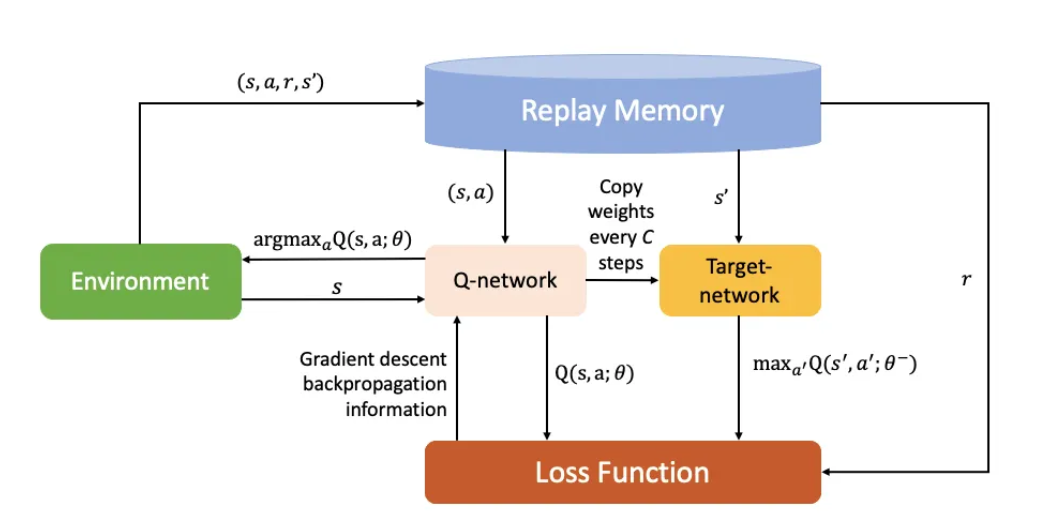
\includegraphics[width=0.85\textwidth]{DRL.png}
\caption{Architecture du Deep Q-Network (DQN)}
\end{figure}

Le DQN introduit un réseau de neurones pour approximer la fonction $Q(s,a;\theta)$ \cite{mnih2015}.

\subsubsection{Principe de fonctionnement}

Le DQN fonctionne selon les étapes suivantes :
\begin{enumerate}
    \item Observation de l’état $s$
    \item Sélection de l’action $a$
    \item Réception de la récompense $r$ et du nouvel état $s'$
    \item Stockage de l’expérience $(s,a,r,s')$ dans la replay memory
    \item Entraînement du réseau à partir d’un mini-batch
\end{enumerate}

\subsubsection{Stabilité de l’apprentissage}

Pour stabiliser l’apprentissage, deux mécanismes sont utilisés :
\begin{itemize}
    \item \textbf{Replay Memory} La replay memory est une mémoire qui stocke les expériences de l’agent sous forme de tuples $(s, a, r, s')$. Au lieu d’apprendre uniquement à partir des expériences récentes, l’agent échantillonne aléatoirement des mini-batchs à partir de cette mémoire.

    Cette technique permet de réduire la corrélation entre les données, d’améliorer l’efficacité de l’apprentissage et d’éviter le phénomène d’oubli des expériences passées. \\
    
    \item \textbf{Target Network} Le target network est une copie du réseau principal, utilisée pour calculer les valeurs cibles dans l’équation de Bellman. Contrairement au réseau principal, ses paramètres sont mis à jour périodiquement.

    Cela permet de stabiliser l’apprentissage en évitant que les valeurs cibles ne changent trop rapidement, ce qui pourrait entraîner des oscillations ou une divergence du modèle.
\end{itemize}

\subsubsection{Bellman Equation}

Le Deep Q-Network (DQN) repose sur l’équation de Bellman pour estimer les valeurs optimales des actions. La valeur cible est définie comme suit :

\begin{equation}
y = r + \gamma \max_{a'} Q(s', a'; \theta^{-})
\end{equation}

Cette équation exprime que la valeur d’une action dépend de la récompense immédiate ainsi que de la meilleure récompense future possible.

\subsubsection{Lien avec la fonction de perte}

L’apprentissage du DQN consiste à minimiser l’erreur entre la valeur estimée et la valeur cible :

\begin{equation}
L(\theta) = \left( r + \gamma \max_{a'} Q(s', a'; \theta^{-}) - Q(s, a; \theta) \right)^2
\end{equation}

où :
\begin{itemize}
    \item $\theta$ représente les poids du réseau principal (Q-network),
    \item $\theta^{-}$ représente les poids du target network,
    \item $s$ est l’état courant,
    \item $a$ est l’action choisie,
    \item $r$ est la récompense obtenue,
    \item $s'$ est l’état suivant,
    \item $\max_{a'} Q(s',a')$ correspond à la meilleure valeur d’action dans l’état suivant.
\end{itemize}

Cette formulation permet au modèle d’apprendre progressivement une approximation optimale de la fonction $Q(s,a)$.

\subsubsection{Pseudo-code du Deep Q-Network (DQN)}

\begin{algorithm}[H]
\caption{Deep Q-Network (DQN)}
\begin{algorithmic}[1]

\STATE Initialiser la replay memory $D$
\STATE Initialiser le Q-network avec des poids aléatoires $\theta$
\STATE Initialiser le target network avec $\theta^{-} = \theta$

\FOR{chaque épisode}
    \STATE Initialiser l’état $s$
    
    \FOR{chaque étape $t$}
    
        \STATE Choisir une action $a$ selon une politique $\epsilon$-greedy
        
        \STATE Exécuter l’action $a$ et observer la récompense $r$ et le nouvel état $s'$
        
        \STATE Stocker $(s, a, r, s')$ dans la replay memory $D$
        
        \STATE Échantillonner un mini-batch aléatoire depuis $D$
        
        \FOR{chaque expérience $(s,a,r,s')$ du mini-batch}
            \STATE Calculer la valeur cible :
            \[
            y = r + \gamma \max_{a'} Q(s', a'; \theta^{-})
            \]
        \ENDFOR
        
        \STATE Mettre à jour les poids $\theta$ en minimisant :
        \[
        L(\theta) = (y - Q(s,a;\theta))^2
        \]
        
        \STATE Mettre à jour l’état : $s \leftarrow s'$
        
        \IF{chaque $C$ étapes}
            \STATE Mettre à jour le target network : $\theta^{-} \leftarrow \theta$
        \ENDIF
        
    \ENDFOR
\ENDFOR

\end{algorithmic}
\end{algorithm}


\subsubsection{Application au Computation Offloading}

Dans le contexte de l’Edge Computing, le DRL permet d’optimiser dynamiquement les décisions de task offloading en tenant compte de l’état du système (ressources, réseau, énergie), afin de minimiser la latence et la consommation énergétique \cite{li2018mec}.

\section{Multi-Agent Reinforcement Learning (MARL)}

Le Multi-Agent Reinforcement Learning (MARL) étend le Reinforcement Learning aux environnements où plusieurs agents interagissent simultanément dans un environnement partagé \cite{albrecht2024marl}. Chaque agent apprend une politique optimale en fonction de ses observations, de ses actions et des interactions avec les autres agents.

Contrairement au RL classique, où l’environnement est supposé stationnaire, le MARL introduit une dynamique non stationnaire, puisque les politiques des agents évoluent simultanément \cite{albrecht2024marl}. Cette interaction rend le processus d’apprentissage plus complexe.

Dans un système multi-agent, les actions des agents sont combinées sous forme d’action jointe, influençant la transition de l’environnement et les récompenses reçues. Ainsi, chaque agent doit apprendre non seulement à interagir avec l’environnement, mais aussi à coordonner ses actions avec les autres agents.

Les interactions entre agents peuvent être de différents types :
\begin{itemize}
    \item Coopératives : les agents partagent un objectif commun,
    \item Compétitives : les agents ont des objectifs opposés,
    \item Mixtes : combinaison de coopération et de compétition.
\end{itemize}

\subsection{Training and Execution Modes in MARL}

Les approches de l’apprentissage multi-agent peuvent être classées selon trois paradigmes principaux : le \textit{Centralized Training and Execution} (CTE), le \textit{Decentralized Training and Execution} (DTE), et le \textit{Centralized Training with Decentralized Execution} (CTDE) \cite{zhang2021marl}.

\subsubsection{Centralized Training and Execution (CTE)}

Dans ce paradigme, l’apprentissage et l’exécution sont entièrement centralisés. Un agent central a accès à l’état global et aux actions de tous les agents, et prend des décisions sous forme d’actions conjointes.

Bien que cette approche permette une coordination optimale, elle souffre d’un problème de scalabilité dû à l’explosion combinatoire de l’espace des actions \cite{zhang2021marl}.

\subsubsection{Decentralized Training and Execution (DTE)}

Dans ce cas, chaque agent apprend et agit de manière indépendante en utilisant uniquement ses observations locales. Cette approche est simple et scalable, mais elle limite fortement la coordination entre agents et peut conduire à des performances sous-optimales \cite{zhang2021marl}.

\subsubsection{Centralized Training with Decentralized Execution (CTDE)}

Le paradigme CTDE combine les avantages des deux approches précédentes. Pendant la phase d’apprentissage, les agents ont accès à des informations globales, ce qui facilite la coordination et réduit les effets de non-stationnarité. En revanche, lors de l’exécution, chaque agent agit de manière autonome en utilisant uniquement ses observations locales \cite{zhang2021marl}.

\begin{figure}[H]
\centering
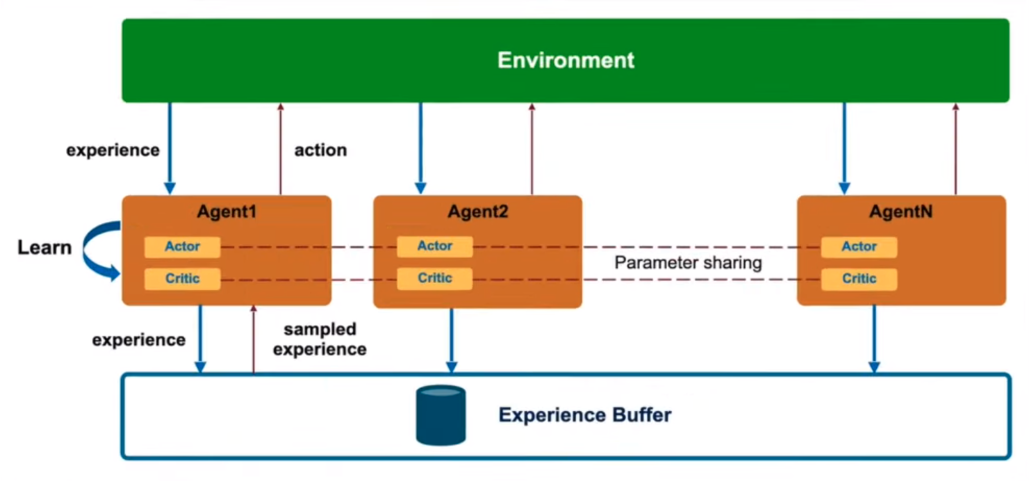
\includegraphics[width=0.9\textwidth]{centralse.png}
\caption{Architecture CTDE : entraînement centralisé avec partage de paramètres et buffer global, suivi d’une exécution décentralisée.}
\end{figure}

Cette approche est aujourd’hui largement utilisée dans les systèmes multi-agents complexes, notamment dans les environnements Edge-IoT, en raison de son équilibre entre performance et scalabilité. Elle permet notamment de :
\begin{itemize}
    \item améliorer la coordination entre agents,
    \item réduire les effets de non-stationnarité,
    \item faciliter l’apprentissage dans des environnements complexes,
    \item conserver une exécution distribuée adaptée aux systèmes Edge et IoT.
\end{itemize}

\subsection{Défis du MARL}

Malgré ses avantages, le MARL présente plusieurs défis majeurs \cite{albrecht2024marl}:

\begin{itemize}
    \item \textbf{Non-stationnarité} : due à l’apprentissage simultané des agents,
    \item \textbf{Coordination} : nécessité d’aligner les actions des agents,
    \item \textbf{Credit assignment} : difficulté d’attribuer une récompense à un agent spécifique,
    \item \textbf{Scalabilité} : explosion combinatoire des actions avec le nombre d’agents.
\end{itemize}

Ainsi, le MARL constitue une approche puissante pour modéliser et résoudre les problèmes distribués complexes, notamment dans les systèmes IoT et Edge Computing.

\section{Travaux existants}

Plusieurs travaux récents ont proposé des approches basées sur le Reinforcement Learning (RL) et le Multi-Agent Reinforcement Learning (MARL) pour résoudre le problème du task offloading dans les environnements Edge Computing.

Par exemple, Baccour et al. \cite{baccour2024} proposent une approche basée sur le MARL afin d’optimiser l’inférence distribuée tout en garantissant la confidentialité des données. Leur solution permet de distribuer dynamiquement les modèles de réseaux de neurones sans recours à un serveur central, en considérant chaque dispositif comme un agent autonome. Les résultats montrent une amélioration des performances en termes de latence et de protection des données.

Dans le même contexte, RL-PDNN \cite{rlpdnn2021} introduit une approche basée sur le Deep Reinforcement Learning (DQN) pour la distribution des réseaux neuronaux, avec un accent particulier sur la sécurité face aux attaques de type white-box. Cette méthode permet une adaptation dynamique des couches du modèle, mais reste limitée dans les environnements multi-agents complexes.

Par ailleurs, Mi et al. \cite{mi2024} proposent un algorithme basé sur le Multi-Agent Deep Reinforcement Learning (MAPPO) pour l’optimisation du task offloading dans des environnements dynamiques. Leur approche s’appuie sur le paradigme CTDE (Centralized Training with Decentralized Execution) et intègre des mécanismes tels que la communication D2D et l’energy harvesting, permettant d’améliorer significativement les performances en termes de latence.

De plus, Hady et al. \cite{marl_resource2025} présentent une étude de synthèse approfondie sur l’utilisation du Multi-Agent Reinforcement Learning pour l’optimisation de l’allocation des ressources dans différents environnements réseau et Edge Computing. Les auteurs analysent les principales approches MARL, leurs architectures, ainsi que les défis liés à la scalabilité, la coopération entre agents, la consommation énergétique et la gestion dynamique des ressources. Cette étude met en évidence l’importance croissante du MARL comme solution efficace pour les systèmes distribués complexes et dynamiques.

Enfin, des études de type survey, telles que \cite{mecsurvey}, mettent en évidence les limites des architectures Cloud traditionnelles, notamment en termes de latence et de bande passante, et justifient l’émergence du Edge Computing comme solution adaptée aux applications IoT.

Cependant, malgré ces avancées, plusieurs limitations persistent. En effet, les approches existantes souffrent souvent de problèmes de non-stationnarité, où l’environnement devient dynamique en raison de l’apprentissage simultané des agents, ce qui complique la convergence des modèles :contentReference. De plus, la scalabilité constitue un défi majeur, car l’espace des actions augmente exponentiellement avec le nombre d’agents, rendant les solutions difficiles à déployer à grande échelle :contentReference.

Par ailleurs, la coordination entre agents reste limitée dans plusieurs approches, et peu de travaux prennent en compte simultanément plusieurs contraintes telles que la latence, l’énergie, la sécurité et la dynamique du réseau. Ces limitations motivent le développement de nouvelles approches basées sur le MARL, capables de gérer efficacement des environnements distribués et complexes.

\subsection{Limites des approches existantes}

Malgré les progrès réalisés, plusieurs limitations importantes persistent dans les travaux existants :

\begin{itemize}
    \item \textbf{Non-stationnarité} : Dans les environnements multi-agents, l’apprentissage simultané des agents rend l’environnement dynamique et instable, ce qui complique la convergence des modèles \cite{zhang2021marl}.  

    \item \textbf{Scalabilité} : L’espace des états et des actions augmente de manière exponentielle avec le nombre d’agents, rendant les modèles difficiles à déployer à grande échelle.  

    \item \textbf{Coordination} : La coordination entre agents reste un défi majeur, notamment dans les scénarios coopératifs ou mixtes.  

    \item \textbf{Hypothèses simplificatrices} : De nombreux travaux reposent sur des modèles réseau simplifiés ou des environnements simulés, ce qui limite leur applicabilité dans des contextes réels.  

    \item \textbf{Manque d’intégration multi-contrainte} : Peu d’approches prennent en compte simultanément la latence, l’énergie, la sécurité et la dynamique du système.  

\end{itemize}

Ainsi, ces limitations justifient la nécessité de développer de nouvelles approches basées sur le MARL, capables de gérer efficacement des environnements dynamiques, distribués et contraints.
\section{Conclusion}

Dans ce chapitre, nous avons présenté un état de l’art des travaux liés au MEC, au computation offloading et aux approches basées sur le RL et le MARL. Nous avons montré que, malgré les progrès réalisés, plusieurs défis persistent, notamment en termes de scalabilité, de coordination et d’adaptabilité.

Ces constats motivent le développement d’une approche basée sur le MARL, qui sera détaillée dans le chapitre suivant.

\chapter{Modélisation et Méthodologie}
\section{Introduction du chapitre}
Dans ce chapitre, nous présentons la modélisation du problème de computation offloading dans un environnement Edge-IoT ainsi que la méthodologie adoptée pour sa résolution. Nous définissons les composants du système, la formulation du problème en tant que processus de décision, ainsi que l’approche basée sur le Multi-Agent Reinforcement Learning (MARL).

\section{Modélisation du système}

\subsection{Architecture du système et environnement}

Le système considéré modélise un environnement de calcul distribué (\textit{Task Offloading}), dans lequel des tâches complexes, telles que l’inférence de modèles de Deep Learning, doivent être exécutées de manière optimale sous des contraintes strictes de latence, d’énergie et de sécurité.

\begin{figure}[H]
    \centering
    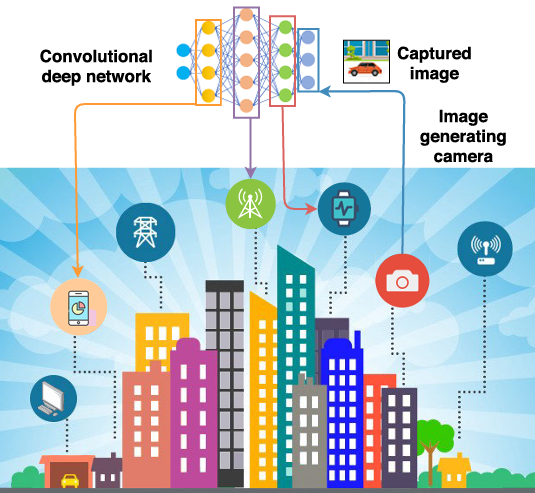
\includegraphics[width=0.9\textwidth]{arch.png}
    \caption{Architecture du système de computation offloading dans un environnement IoT distribué. 
    Les dispositifs IoT jouent un double rôle : agents générant les tâches (sources de données) et nœuds de calcul contraints participant à l’exécution distribuée des modèles de Deep Learning.}
    \label{fig:system_model}
\end{figure}

\begin{itemize}
    \item \textbf{Devices IoT} :
    Comme illustré dans la Figure~\ref{fig:system_model}, les dispositifs IoT constituent les entités principales du système et sont interconnectés au sein d’un environnement distribué.  
    L’ensemble des dispositifs disponibles forme un pool de ressources hétérogènes noté $\mathcal{M}$, où chaque dispositif $m \in \mathcal{M}$ est caractérisé par sa fréquence CPU $F_m$, sa bande passante $BW_m$, sa capacité mémoire $C^{mem}_m$, son budget énergétique $B_m$ et son score de confiance $sl_m$.
    
    Dans notre modélisation, les dispositifs IoT sont divisés en deux catégories selon leur rôle :

    \begin{itemize}
        \item \textbf{Devices IoT en tant qu’agents (sources de données)} :  
        Ces dispositifs représentent les utilisateurs ou les sources de requêtes. Ils génèrent des données et initient des tâches d’inférence. 
        Chaque dispositif est modélisé comme un agent autonome $n \in \mathcal{N}$, capable de prendre des décisions concernant l’exécution locale ou le déchargement (\textit{offloading}) des tâches.

        \item \textbf{Devices IoT en tant que nœuds de calcul contraints} :  
        Certains dispositifs IoT peuvent également être utilisés comme des ressources de calcul limitées. 
        Ces nœuds correspondent à un sous-ensemble des ressources $m \in \mathcal{M}$ et sont caractérisés par des contraintes strictes en termes de :
        \begin{itemize}
            \item capacité de calcul (liée à $F_m$),
            \item mémoire disponible ($C^{mem}_m$),
            \item budget énergétique ($B_m$),
            \item niveau de confidentialité et de sécurité ($sl_m$).
        \end{itemize}
        Leur participation à l’exécution des tâches dépend de la disponibilité de leurs ressources et des exigences des tâches.
    \end{itemize}
\end{itemize}

\subsection{Modélisation des tâches}

Chaque agent $n \in \mathcal{N}$ génère une tâche correspondant à l’inférence d’un modèle de Deep Learning.

Cette tâche est modélisée comme une séquence de couches $\mathcal{L}_n = \{1, 2, ..., L\}$, où chaque couche $l$ représente une sous-tâche caractérisée par :
\begin{itemize}
    \item un coût de calcul (FLOPS),
    \item un besoin mémoire,
    \item une taille de données de sortie $D_{n,l}$,
    \item un niveau de confidentialité.
\end{itemize}

\begin{figure}[H]
    \centering
    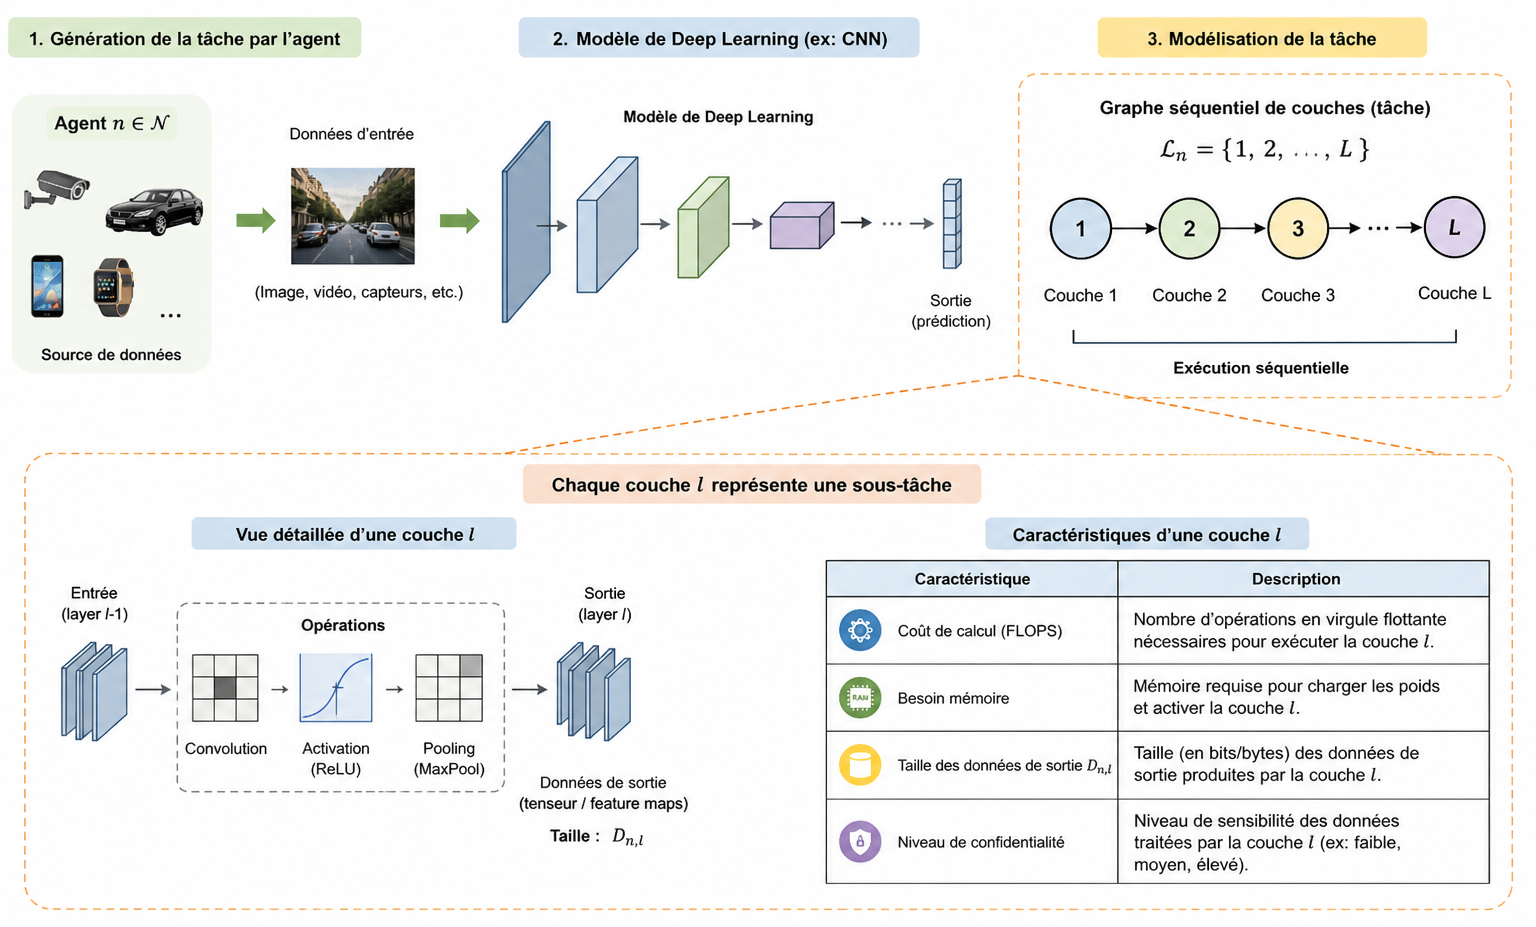
\includegraphics[width=\textwidth]{task_model.png}
    \caption{Modélisation d’une tâche de Deep Learning comme une séquence de sous-tâches (couches).}
    \label{fig:task_model}
\end{figure}

Comme illustré dans la Figure~\ref{fig:task_model}, les données d’entrée sont traitées par un modèle de Deep Learning composé de plusieurs couches successives. Chaque couche applique des opérations telles que la convolution, l’activation (ReLU) et le pooling, produisant des données intermédiaires utilisées par la couche suivante.

Dans ce travail, nous considérons des modèles CNN organisés sous forme d’un pipeline séquentiel.

Le coût de calcul d’une couche convolutionnelle (Convolution Layer) est donné par :

\begin{equation}
c_{n,l} = n_{l-1} \cdot S_l \cdot n_l \cdot o_l
\end{equation}

où :
\begin{itemize}
    \item $n_{l-1}$ est le nombre de canaux d’entrée de la couche $l$,
    \item $S_l$ représente la taille spatiale du filtre (ex: $k \times k$),
    \item $n_l$ est le nombre de filtres (ou canaux de sortie),
    \item $o_l$ est la taille spatiale de la carte de sortie.
\end{itemize}

Cette expression correspond au nombre total d’opérations nécessaires pour effectuer les convolutions, ce qui permet d’estimer la charge de calcul de la couche.

\vspace{0.3cm}

Pour une couche entièrement connectée (Fully-Connected layer), le coût de calcul est donné par :

\begin{equation}
c_{n,l} = n_{l-1}^* \cdot n_l^*
\end{equation}

où :
\begin{itemize}
    \item $n_{l-1}^*$ est le nombre de neurones en entrée,
    \item $n_l^*$ est le nombre de neurones en sortie.
\end{itemize}

Ce coût correspond au nombre de multiplications nécessaires pour relier chaque neurone d’entrée à chaque neurone de sortie.

\vspace{0.3cm}

La mémoire requise par une couche est définie par :

\begin{equation}
m_{n,l} = W_{n,l} \cdot b
\end{equation}

où :
\begin{itemize}
    \item $W_{n,l}$ est le nombre total de poids (paramètres) de la couche,
    \item $b$ est le nombre de bits utilisés pour représenter chaque poids.
\end{itemize}

Cette quantité représente la mémoire nécessaire pour stocker les paramètres du modèle, ce qui est un facteur critique dans les environnements IoT contraints.\\

Les couches de type pooling et ReLU introduisent un coût négligeable. Enfin, les données de sortie $O_j^k$ générées par chaque couche sont transmises à la suivante, ce qui influence directement le coût de communication en cas d’offloading.

Ainsi, cette modélisation permet de décomposer une tâche complexe en sous-tâches distribuables, facilitant l’optimisation de l’exécution dans un environnement Edge-IoT.

\subsection{Modèle de latence}

La latence totale d’une tâche dépend du temps de calcul, du temps de communication ainsi que des délais d’attente dus à la congestion des ressources.

\paragraph{Temps de calcul}

Le temps de calcul pour exécuter une couche $l$ sur un dispositif $m$ est donné par :

\begin{equation}
T_{comp}(n,l,m) = \frac{C_{n,l}}{f_m} + W_{comp}^m(n,t)
\end{equation}

où :
\begin{itemize}
    \item $n \in \mathcal{N}$ représente l’agent ou la tâche générée par un dispositif IoT,
    \item $l \in \mathcal{L}_n$ représente la couche du modèle de Deep Learning associée à la tâche $n$,
    \item $m \in \mathcal{M}$ représente le dispositif de calcul sélectionné pour exécuter la couch,
    \item $C_{n,l}$ est la charge de calcul (FLOPS),
    \item $f_m$ est la fréquence du processeur,
    \item $W_{comp}^m(n,t)$ est le délai d’attente dû à la congestion du CPU.
\end{itemize}

\paragraph{File d’attente (Queuing Delay)}

Dans un environnement multi-agent, plusieurs tâches peuvent être envoyées vers le même dispositif. Cela engendre un délai d’attente :

\begin{equation}
W_{comp}^m(n,t) = \sum_{\substack{n' \neq n}} \sum_{l'} A_{n',l'}^m \cdot \frac{C_{n',l'}}{f_m}
\end{equation}

Ce terme permet de modéliser la congestion et incite les agents à équilibrer la charge entre les dispositifs.

\paragraph{Temps de communication}

\begin{equation}
T_{comm}(n,l,m',m) =
\begin{cases}
0 & \text{si } m = m' \\
\frac{D_{n,l-1}}{BW_m} + W_{comm}^m(n,t) & \text{sinon}
\end{cases}
\end{equation}

où $W_{comm}^m(n,t)$ représente le délai dû à la congestion du réseau.

\paragraph{Latence totale}

\begin{equation}
T_n = \sum_{l \in \mathcal{L}_n} \sum_{m \in \mathcal{M}} A_{n,l}^m 
\left( T_{comp}(n,l,m) + \sum_{m'} A_{n,l-1}^{m'} \cdot T_{comm}(n,l,m',m) \right)
\end{equation}

\subsection{Dynamic Voltage and Frequency Scaling (DVFS)}

Le \textit{Dynamic Voltage and Frequency Scaling} (DVFS) est une technique de gestion énergétique largement utilisée dans les processeurs modernes afin de réduire la consommation électrique et la dissipation thermique tout en maintenant un niveau de performance acceptable \cite{suleiman_dvfs, wu2005dvfs}.

Le principe du DVFS consiste à ajuster dynamiquement :
\begin{itemize}
    \item la fréquence d’horloge du processeur,
    \item la tension d’alimentation,
\end{itemize}
en fonction de la charge de travail du système.

\subsubsection{Fonctionnement du DVFS}

Le mécanisme de \textit{Dynamic Voltage and Frequency Scaling} (DVFS) permet d’ajuster dynamiquement la fréquence du processeur en appliquant un facteur de réduction à la fréquence maximale du CPU \cite{lesueur2010dvfs}.

\paragraph{Charge faible}

Lorsque le processeur exécute des tâches légères ou lorsque la charge du système est faible :
\begin{itemize}
    \item la fréquence du processeur diminue ;
    \item la tension d’alimentation diminue également.
\end{itemize}

Cette réduction simultanée permet de :
\begin{itemize}
    \item diminuer la consommation énergétique ;
    \item réduire la dissipation thermique et l’échauffement du processeur.
\end{itemize}

\paragraph{Charge élevée}

Lorsque le système doit traiter des calculs intensifs ou des applications exigeantes :
\begin{itemize}
    \item la fréquence du processeur augmente ;
    \item la tension augmente afin de garantir la stabilité du fonctionnement.
\end{itemize}

Dans ce cas, le DVFS favorise :
\begin{itemize}
    \item de meilleures performances computationnelles ;
    \item une exécution plus rapide des tâches.
\end{itemize}

Cependant, cette augmentation entraîne également une consommation énergétique plus importante.

\subsubsection{DVFS et apprentissage par renforcement}

Les approches récentes utilisent l’apprentissage par renforcement (\textit{Reinforcement Learning}) afin d’optimiser dynamiquement les décisions DVFS.

Dans ce contexte :
\begin{itemize}
    \item l’agent observe l’état du système (charge CPU, énergie, température),
    \item choisit une fréquence adaptée,
    \item puis reçoit une récompense basée sur le compromis énergie-performance.
\end{itemize}

Cette approche permet d’apprendre automatiquement une politique optimale dans des environnements dynamiques et hétérogènes, tels que les systèmes IoT-Edge.

\subsection{Modèle énergétique avec DVFS}

Afin de modéliser de manière réaliste la consommation énergétique des dispositifs IoT, nous adoptons un modèle basé sur le \textit{Dynamic Voltage and Frequency Scaling} (DVFS), qui permet d’ajuster dynamiquement la fréquence du processeur \cite{lesueur2010dvfs}.

\paragraph{Choix de la fréquence}

Chaque agent ne choisit pas uniquement le dispositif $m$, mais également un ratio de fréquence $\rho \in (0,1]$, tel que :

\begin{equation}
f_{eff} = f_m \cdot \rho
\end{equation}

où :
\begin{itemize}
    \item $f_{eff}$ représente la fréquence effective utilisée ;
    \item $f_{max}$ correspond à la fréquence maximale du processeur ;
    \item $\rho \in (0,1]$ désigne le facteur de scaling appliqué par le système.
\end{itemize}

Lorsque le facteur $\rho$ est proche de $1$, le processeur fonctionne à une fréquence élevée afin d’offrir de meilleures performances. En revanche, lorsque ce facteur diminue, la fréquence du processeur est réduite, ce qui permet de diminuer la consommation énergétique et la dissipation thermique.

\paragraph{Simplification avec DVFS}
Dans les circuits CMOS, la puissance dynamique consommée par un processeur est donnée par :

\begin{equation}
P_{dyn} = \kappa \cdot V^2 \cdot f
\end{equation}

où :
\begin{itemize}
    \item $A$ est le facteur d’activité des transistors,
    \item $C$ est la capacité effective de commutation,
    \item $V$ est la tension d’alimentation,
    \item $f$ est la fréquence du processeur.
\end{itemize}

Cette équation montre que la consommation énergétique dépend quadratiquement de la tension et linéairement de la fréquence.

En pratique, lorsque la fréquence est réduite, la tension peut également être diminuée proportionnellement, ce qui conduit à supposer une relation linéaire entre la tension et la fréquence, telle que :

\begin{equation}
V \propto f
\end{equation}

En remplaçant cette relation dans le modèle de consommation dynamique, on obtient un modèle cubique simplifié :

\begin{equation}
P_{comp} = \kappa \cdot f^3
\end{equation}

où $\kappa$ représente un coefficient dépendant des caractéristiques matérielles du processeur.

\paragraph{Temps de calcul avec DVFS}

La réduction de la fréquence augmente le temps de calcul :

\begin{equation}
T_{comp}(n,l,m) = \frac{C_{n,l}}{f_{eff}}
\end{equation}

\paragraph{Énergie de calcul}

\begin{equation}
E_{comp}(n,l,m) = P_{comp} \cdot T_{comp}(n,l,m)
\end{equation}

\paragraph{Énergie de communication}

\begin{equation}
E_{comm}(n,l,m',m) = P_m^{comm} \cdot T_{comm}(n,l,m',m)
\end{equation}

\paragraph{Énergie totale}

\begin{equation}
E_n = \sum_{l \in \mathcal{L}_n} \sum_{m \in \mathcal{M}} A_{n,l}^m 
\left( E_{comp}(n,l,m) + \sum_{m'} A_{n,l-1}^{m'} \cdot E_{comm}(n,l,m',m) \right)
\end{equation}

\paragraph{Compromis latence-énergie}

Le modèle DVFS introduit un compromis fondamental :

\begin{itemize}
    \item Réduire la fréquence ($\rho \downarrow$) augmente le temps de calcul (latence plus élevée),
    \item mais réduit fortement la puissance consommée ($\propto f^3$),
    \item ce qui diminue significativement l’énergie totale consommée.
\end{itemize}

Par exemple, si la fréquence est divisée par deux, la latence est multipliée par deux, tandis que la puissance est divisée par huit, ce qui réduit l’énergie globale d’un facteur quatre.

Ce compromis rend le problème particulièrement complexe et justifie l’utilisation d’approches d’apprentissage par renforcement pour apprendre une politique optimale.

\subsection{Modèle mathématique du système}

Afin de formaliser le problème de computation offloading dans l’environnement IoT distribué décrit précédemment, nous introduisons une modélisation mathématique du système.

\subsubsection{Objectif global}

L’objectif principal du système est d’optimiser l’allocation et l’exécution des tâches dans un environnement IoT distribué, en tenant compte des contraintes de ressources limitées et des exigences de performance.

Plus précisément, il s’agit de :

\begin{itemize}
    \item \textbf{Minimiser la latence} : réduire le temps total d’exécution des tâches, incluant les délais de calcul et de communication.
    \item \textbf{Minimiser la consommation énergétique} : limiter l’énergie consommée par les dispositifs, en particulier pour les équipements IoT à batterie limitée.
    \item \textbf{Maximiser la performance} : améliorer le temps de réponse global et la qualité de service.
    \item \textbf{Optimiser l’utilisation des ressources} : équilibrer la charge entre les dispositifs afin d’éviter la congestion et la sous-utilisation.
\end{itemize}

\subsubsection{Ensemble des dispositifs}

Le système est composé d’un ensemble de dispositifs hétérogènes noté :

\begin{equation}
\mathcal{M} = \{1, 2, ..., M\}
\end{equation}

Chaque dispositif $m$ est caractérisé par les paramètres suivants :

\begin{itemize}
    \item Fréquence CPU : $F_m$
    \item Bande passante : $BW_m$
    \item Capacité mémoire : $C^{mem}_m$
    \item Budget énergétique : $B_m$
    \item Score de confiance : $sl_m$
\end{itemize}
Nous supposons que tous les dispositifs utilisent la même technologie de communica-
tion, mais avec des débits de transmission différents $\rho_i$. De plus, tous les dispositifs sont connectés et peuvent communiquer entre eux.

\subsubsection{Ensemble des agents}

Les dispositifs générant les tâches sont modélisés comme un ensemble d’agents :

\begin{equation}
\mathcal{N} = \{1, 2, ..., N\}
\end{equation}

Chaque agent $n \in \mathcal{N}$ génère une tâche d’inférence.

\subsubsection{Modélisation des tâches}

Une tâche générée par un agent $n$ est représentée comme une séquence de couches :

\begin{equation}
\mathcal{L}_n = \{1, 2, ..., L_n\}
\end{equation}

Chaque couche $l \in \mathcal{L}_n$ est caractérisée par :

\begin{itemize}
    \item Coût de calcul : $c_{n,l}$
    \item Besoin mémoire : $m_{n,l}$
    \item Taille des données de sortie : $D_{n,l}$
    \item Niveau de confidentialité : $\sigma_{n,l}$
\end{itemize}

\subsubsection{Formulation mathématique de l’objectif}

Ces objectifs sont modélisés sous forme d’un problème d’optimisation multi-objectif, combinant la latence et la consommation énergétique :

\begin{equation}
\min_{\mathbf{a}} \sum_{n \in \mathcal{N}} \left( \alpha T_n + \beta E_n \right)
\end{equation}

où :
\begin{itemize}
    \item $T_n$ représente la latence totale de la tâche $n$,
    \item $E_n$ représente la consommation énergétique associée,
    \item $\alpha$ et $\beta$ sont des coefficients de pondération permettant d’ajuster l’importance relative de chaque objectif.
\end{itemize}

\subsubsection{Contraintes du problème}

Le problème d’allocation des tâches est soumis à plusieurs contraintes garantissant la faisabilité du système et le respect des limitations physiques et de sécurité.

\paragraph{(1.a) Contrainte d’affectation unique}

\begin{equation}
\sum_{i \in \mathcal{I} \cup s_n} A_{n,l}^{i} =
\begin{cases}
1 & \text{si } l \leq L_r \\
0 & \text{sinon}
\end{cases}
\end{equation}

où :
\begin{itemize}
    \item $A_{n,l}^{i}$ est une variable binaire indiquant si la couche $l$ de la tâche $n$ est exécutée sur le dispositif $i$,
    \item $\mathcal{I}$ représente l’ensemble des dispositifs disponibles,
    \item $s_n$ représente le dispositif source associé à la tâche $n$,
    \item $L_r$ est le nombre total de couches du modèle.
\end{itemize}

Cette contrainte garantit que chaque couche est exécutée sur un seul dispositif afin d’éviter toute duplication de calcul.

\paragraph{(1.b) Contrainte de mémoire}

\begin{equation}
\sum_{n \in \mathcal{N}} \sum_{l \in \mathcal{L}_n} A_{n,l}^m \cdot m_{n,l}
\leq C^{mem}_m
\quad \forall m \in \mathcal{M}
\end{equation}

où :
\begin{itemize}
    \item $m_{n,l}$ représente la mémoire requise par la couche $l$,
    \item $C^{mem}_m$ est la capacité mémoire disponible du dispositif $m$.
\end{itemize}

Cette contrainte impose que la mémoire totale consommée ne dépasse pas la mémoire disponible du dispositif.

\paragraph{(1.c) Contrainte de capacité de calcul}

\begin{equation}
\sum_{n \in \mathcal{N}} \sum_{l \in \mathcal{L}_n} A_{n,l}^m \cdot c_{n,l}
\leq \overline{C}_m
\quad \forall m \in \mathcal{M}
\end{equation}

où :
\begin{itemize}
    \item $c_{n,l}$ représente le coût computationnel de la couche $l$,
    \item $\overline{C}_m$ est la capacité maximale de calcul du dispositif $m$.
\end{itemize}

Cette contrainte garantit que la charge de calcul totale ne dépasse pas les ressources disponibles du dispositif.

\paragraph{(1.d) Contrainte énergétique}

\begin{equation}
E_m^{total} \leq B_m
\quad \forall m \in \mathcal{M}
\end{equation}

où :
\begin{itemize}
    \item $E_m^{total}$ représente l’énergie totale consommée par le dispositif $m$,
    \item $B_m$ représente le budget énergétique disponible.
\end{itemize}

Cette contrainte empêche l’épuisement énergétique des dispositifs IoT.

\paragraph{(1.e) Contrainte de confidentialité et de confiance}

\begin{equation}
\sigma_m \geq \sigma_{min} \cdot \frac{\sigma_{n,l}}{\sigma_{max}}
\end{equation}

où :
\begin{itemize}
    \item $\sigma_m$ représente le niveau de confiance du dispositif $m$,
    \item $\sigma_{n,l}$ représente le niveau de confidentialité requis par la couche $l$,
    \item $\sigma_{min}$ et $\sigma_{max}$ représentent respectivement les niveaux minimal et maximal de sécurité.
\end{itemize}

Cette contrainte garantit qu’une couche sensible ne peut être exécutée que sur un dispositif suffisamment sécurisé.

\paragraph{(1.f) Contrainte de sécurité (exposition)}

\begin{equation}
\sum_{l \in \mathcal{L}_n} A_{n,l}^m
\leq
\left\lfloor L_n \cdot S \right\rfloor
\quad \forall n \in \mathcal{N}, \forall m \in \mathcal{M}
\end{equation}

où :
\begin{itemize}
    \item $L_n$ représente le nombre total de couches du modèle,
    \item $S \in (0,1]$ représente la fraction maximale autorisée des couches pouvant être exposées à un même dispositif.
\end{itemize}

Le terme :

\begin{equation}
\sum_{l \in \mathcal{L}_n} A_{n,l}^m
\end{equation}

représente le nombre total de couches exécutées sur le dispositif $m$.

Cette contrainte limite l’exposition d’un modèle complet à un seul dispositif afin de réduire les risques d’attaques de type \textit{white-box}.

\paragraph{(1.g) Contrainte de bande passante}

\begin{equation}
\sum_{i \in \mathcal{M}}
\sum_{n \in \mathcal{N}}
\sum_{l \in \mathcal{L}_n}
A_{n,l-1}^{i} \cdot A_{n,l}^{j} \cdot D_{n,l}
\leq BW_m
\quad \forall m \in \mathcal{M}
\end{equation}

où :
\begin{itemize}
    \item $D_{n,l}$ représente la taille des données transmises,
    \item $BW_m$ représente la bande passante disponible du dispositif $m$.
\end{itemize}

Cette contrainte garantit que les transmissions réseau ne dépassent pas la capacité disponible.

\paragraph{(1.h) Contrainte de diversité séquentielle}

\begin{equation}
A_{n,l}^{m} + A_{n,l-1}^{m} \leq 1
\quad
\forall n \in \mathcal{N},
\forall l > 1,
\forall m \in \mathcal{M}
\end{equation}

Cette contrainte impose que deux couches consécutives d’une même tâche ne soient pas exécutées sur le même dispositif.

Elle favorise la distribution des calculs sur plusieurs nœuds afin d’améliorer la sécurité et l’équilibrage de charge.

\subsubsection{Complexité et résolution}

Le problème formulé est un problème d’optimisation combinatoire de type \textit{Mixed-Integer Non-Linear Programming} (MINLP), caractérisé par :

\begin{itemize}
    \item un espace de décision discret (variables binaires $A_{n,l}^m$),
    \item des relations non linéaires (latence et énergie),
    \item des contraintes multiples et interdépendantes.
\end{itemize}

Ce type de problème est connu pour être NP-difficile, ce qui rend la recherche d’une solution optimale exacte impraticable dans des environnements dynamiques et en temps réel.

Par conséquent, au lieu de recourir à des méthodes d’optimisation classiques, nous reformulons le problème comme un processus de décision markovien (MDP) et adoptons une approche basée sur l’apprentissage par renforcement multi-agent (MARL), permettant d’apprendre des politiques d’allocation efficaces de manière adaptative.

\chapter{Résultats et Discussion}
\chapter{Conclusion et Perspectives}

















\newpage
\printbibliography

\end{document}